\documentclass[12pt, a4paper, oneside]{book}

%\usepackage{fullpage}
%\usepackage{amsmath}
%\usepackage{amssymb}
\usepackage{graphicx}
%\usepackage{alltt}
%\usepackage{latexsym}
%\usepackage{url}
%\usepackage[iso]{umlaute}
%\usepackage[arrow,matrix,frame,curve,ps]{xy}
\usepackage[vcentering,dvips]{geometry}
%\usepackage{xypic}
%\usepackage[iso]{umlaute}
%\usepackage{amssymb}
%\usepackage{fleqn}
%\usepackage{alltt,epsfig,array}
\usepackage{listings}
\usepackage[labelfont=bf,up,textfont=it,up]{caption}
\usepackage{algorithmic}
\usepackage{algorithm}
\usepackage{setspace}
%\usepackage{makeidx}
%\usepackage{float}
%\usepackage{array}
\usepackage{verbatim}
\usepackage[
	pdftex,
	plainpages=false,
	pdfpagelabels,
	colorlinks=false,
	pdftitle={Keyboard Supported Diagram Editing and Navigating},    % title
	pdfsubject={Bachelor Thesis},
	pdfauthor={Andrew M. B. Boktor},     % author
	pdfkeywords={diagram keyboard editing edit creation create navigation navigate accessibility accessibilities}
]{hyperref}

\geometry{total={155mm,235mm}}

%\setlength{\parindent}{0pt}

\thispagestyle{plain}

%Create your own environments
%%%%%%%%%%%%%%%%%%%%%%%%%%%%%% inclusion commands %%%%%%%%%%%%%%%%%%%%%%%%%%%%%%%%%%
\newtheorem{definition}{Definition}
\newtheorem{example}{Example}

\newcommand{\reffig}[1]{
{\em Figure~\ref{figure:#1}}\noindent
}

\newcommand{\incfig}[4]{%
	\begin{figure}[hHtb!]
		\begin{center}
			\includegraphics[#4]{illustrations/#1}
			\caption{#2}
			\label{figure:#3}
		\end{center}
	\end{figure}
}

\newcommand{\inctext}[3]{
	\begin{figure}
		{#1}
		\caption{#2}
		\label{figure:#3}
	\end{figure}
}

\newcommand{\inccode}[3]{
	\begin{figure}[hHtb!]
	\lstset{basicstyle=\footnotesize, numberstyle=\footnotesize, numbers=left, frame=single, tabsize=2}
	\lstinputlisting{code/#1}
	\caption{#2}
	\label{figure:#3}
	\end{figure}
}

\newcommand{\refcode}[1]{
{\em Figure~\ref{figure:#1}}\noindent
}

\newcommand{\labelchapter}[1]{
\label{chapter:#1}
}
\newcommand{\refchapter}[1]{
{\em Chapter~\ref{chapter:#1}}\noindent
}

\newcommand{\labelsection}[1]{
\label{section:#1}
}
\newcommand{\refsection}[1]{
{\em Section~\ref{section:#1}}\noindent
}

\newcommand{\labelsubsection}[1]{
\label{subsection:#1}
}
\newcommand{\refsubsection}[1]{
{\em Section~\ref{subsection:#1}}\noindent
}

\newcommand{\labeltable}[1]{
\label{table:#1}
}
\newcommand{\reftable}[1]{
{\em Table~\ref{table:#1}}\noindent
}

\newcommand{\labelappendix}[1]{
\label{appendix:#1}
}
\newcommand{\refappendix}[1]{
{\em Appendix~\ref{appendix:#1}}\noindent
}

%%%%%%%%%%%%%%%%%%%%%%%%%%%% Thesis Specific Commands %%%%%%%%%%%%%%%%%%%%%%%%%%%%%%
%Submission Date
\newcommand{\submissionDay}[0]{2\superscript{nd}}
\newcommand{\submissionMonth}[0]{September}
\newcommand{\submissionYear}[0]{2008}
\newcommand{\submissionDate}[0]{\submissionDay~of~\submissionMonth,~\submissionYear}

%Thesis
\newcommand{\typeOfThesis}[0]{Bachelor Thesis}
\newcommand{\titleOfThesisOne}[0]{Keyboard Supported Diagram Editing and Navigating}

%Author and Reviewers
\newcommand{\authorOfThesis}[0]{Andrew M. B. Boktor}
\newcommand{\supervisorOne}[0]{Dipl. Inf. Steffen Koch}
\newcommand{\supervisorTwo}[0]{Dipl. Inf. Christiane Taras}
\newcommand{\reviewerOne}[0]{Prof. Dr. Thomas Ertl}

%%%%%%%%%%%%%%%%%%%%%%%%%%%%%% Formatting Commands %%%%%%%%%%%%%%%%%%%%%%%%%%%%%%%%%
\newcommand{\superscript}[1]{\ensuremath{^{\textnormal{#1}}}}
\newcommand{\subscript}[1]{\ensuremath{_{\textnormal{#1}}}}
\newcommand{\beginchapter}[0]{
\vspace{-0.5cm}
\hrule
\vspace{0.02cm}
\hrule
\vspace{0.01cm}
\hrulefill
\hrule
\hrule
\vspace{1cm}
}

%%%%%%%%%%%%%%%%%%%%%%%%%%%% Document Initialization %%%%%%%%%%%%%%%%%%%%%%%%%%%%%%%
\makeindex
\makeindex

%%%%%%%%%%%%%%%%%%%%%%%%%%%%%%%%%%%%%%%%%%%%%%%%%%%%%%%%%%%%%%%%%%%%%%%%%%%%%%%%%%%%
\begin{document}

\pagenumbering{Roman}

%++++++++++++++++++++++++++++++++++++++++++++++++++++++++++++++++++++
\thispagestyle{empty}
\begin{center}
	\hrule
	\vspace{1cm}
	{\Large \bf Media Engineering and Technology Faculty}\\ %[1mm]
	\vspace{0.3cm}
	{\Large \bf German University in Cairo}\\ %[1mm]
	\begin{figure}[htb]
		\centering
		
\includegraphics[width=2cm]{logos/logo-university-guc.pdf}
		%\label{GUC_LOGO}
	\end{figure}
	
	\vspace{0.4cm}
	
	{\Large \bf Institute of Visualization and Interactive Systems}\\ %[1mm]
	\vspace{0.3cm}
	{\Large \bf University of Stuttgart}\\ %[1mm]

	\begin{figure}[htb]
		\centering
		
\includegraphics[width=2cm]{logos/logo-university-stuttgart.pdf}
		%\label{STUTTGART_LOGO}
		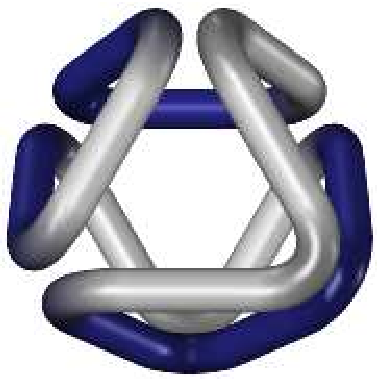
\includegraphics[width=2cm]{logos/logo-university-vis.pdf}
		%\label{VIS_LOGO}
	\end{figure}
	
	\vspace{2cm}
	
	{\Large \bf \titleOfThesisOne}\\
	\vspace{1cm}
	
	{\large \bf \typeOfThesis}\\
	\vspace{4cm}
	
	\parbox{2.5cm}{
		%\begin{large}
			\begin{tabbing}
				Author: \hspace{2cm}
					\=\authorOfThesis\\[2mm]
				Supervisor: 
					\>\supervisorOne\\[2mm]
					\>\supervisorTwo\\[2mm]
				Reviewers: 
					\>\reviewerOne\\[1mm]
				Submission Date: 
					\>\submissionDate\\
			\end{tabbing}
		%\end{large}
	}\\
	\hrule
	%\vspace{0.01cm}
	%\hrule
\end{center}
%++++++++++++++++++++++++++++++++++++++++++++++++++++++++++++++++++++

%++++++++++++++++++++++++++++++++++++++++++++++++++++++++++++++++++++
\thispagestyle{empty}
\begin{center}
	\hrule
	\vspace{1cm}
	{\Large \bf Media Engineering and Technology Faculty}\\ %[1mm]
	\vspace{0.3cm}
	{\Large \bf German University in Cairo}\\ %[1mm]
	\begin{figure}[htb]
		\centering
		
\includegraphics[width=2cm]{logos/logo-university-guc.pdf}
		%\label{GUC_LOGO}
	\end{figure}
	
	\vspace{0.4cm}
	
	{\Large \bf Institute of Visualization and Interactive Systems}\\ %[1mm]
	\vspace{0.3cm}
	{\Large \bf University of Stuttgart}\\ %[1mm]

	\begin{figure}[htb]
		\centering
		
\includegraphics[width=2cm]{logos/logo-university-stuttgart.pdf}
		%\label{STUTTGART_LOGO}
		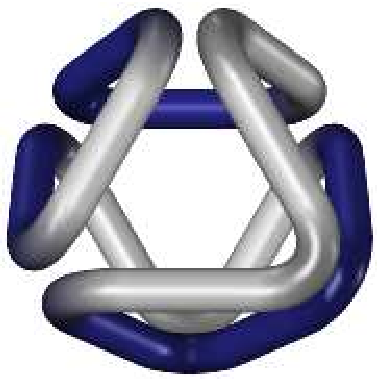
\includegraphics[width=2cm]{logos/logo-university-vis.pdf}
		%\label{VIS_LOGO}
	\end{figure}
	
	\vspace{2cm}
	
	{\Large \bf \titleOfThesisOne}\\
	\vspace{1cm}
	
	{\large \bf \typeOfThesis}\\
	\vspace{4cm}
	
	\parbox{2.5cm}{
		%\begin{large}
			\begin{tabbing}
				Author: \hspace{2cm}
					\=\authorOfThesis\\[2mm]
				Supervisor: 
					\>\supervisorOne\\[2mm]
					\>\supervisorTwo\\[2mm]
				Reviewers: 
					\>\reviewerOne\\[1mm]
				Submission Date: 
					\>\submissionDate\\
			\end{tabbing}
		%\end{large}
	}\\
	\hrule
	%\vspace{0.01cm}
	%\hrule
\end{center}
%++++++++++++++++++++++++++++++++++++++++++++++++++++++++++++++++++++

%++++++++++++++++++++++++++++++++++++++++++++++++++++++++++++++++++++
\thispagestyle{empty}
This is to certify that:
\renewcommand{\labelenumi}{\roman{enumi}.}
\begin{enumerate}
\item the thesis compromises only my original work toward the Bachelor Degree
\item due acknowledgment has been made in the text to all other material used
\end{enumerate}
\renewcommand{\labelenumi}{\arabic{enumi}.}

\vspace{2cm}
\begin{flushright}
\rule[0mm]{6cm}{0.2mm}\\
\authorOfThesis\\
\submissionDate\\
\end{flushright}

\chapter*{Abstract}
\labelchapter{abstract}
%-----------------------
\beginchapter
%-----------------------
The abstract is a very important and obligatory part of the report
allowing the potential reader to judge, if he is the target of this
report.  The abstract should be written with broadly understandable
technical language and should be self-contained, i.e. should not
contain any references or citations. Also the usage of abbreviations
and acronyms should be avoided, since the same acronyms or
abbreviations can have different meanings on different research
fields.  The abstract should typically contain about 300 words and in
any cases not more than one page.  The definition of the research
field and the most important outcome of the presented research are the
obligatory components of the abstract.

\chapter*{Acknowledgments}
%-----------------------
\addcontentsline{toc}{chapter}{Acknowledgments}
\beginchapter
%-----------------------

%%%%%%%%%%%%%%%%%%%%%%%%%%%%%%%%%%%% List Of **** %%%%%%%%%%%%%%%%%%%%%%%%%%%%%%%%%%
\listoftables
\labelchapter{list_of_tables}
%-----------------------
\addcontentsline{toc}{chapter}{List of Tables}
\thispagestyle{plain}
%-----------------------
\listoffigures
%-----------------------
\addcontentsline{toc}{chapter}{List of Figures}
\thispagestyle{plain}
%-----------------------
\chapter*{List of Abbreviations}
%-----------------------
\addcontentsline{toc}{chapter}{List of Abbreviations}
\thispagestyle{plain}
%-----------------------


%%%%%%%%%%%%%%%%%%%%%%%%%%%%%%%%%%%%%%%%%%%%%%%%%%%%%%%%%%%%%%%%%%%%%%%%%%%%%%%%%%%%

\tableofcontents
\clearpage

\pagenumbering{arabic}

%%%%%%%%%%%%%%%%%%%%%%%%%%%%%%%%%%%%%%%%%%%%%%%%%%%%%%%%%%%%%%%%%%%%%
\chapter{Introduction}
%-----------------------
\beginchapter
%-----------------------




The main task of the introduction in the report is to present the
logical chain


\section{Motivation}


\section{Aim of the project}



%\chapter{Technical Background}\label{chap:background}
%-----------------------
\beginchapter
%-----------------------
This chapter will introduce some basic concepts that will be help understand further work done in this thesis.

\section{Graphs}
\chapter{Problem Description}
\labelchapter{problem_description}
%-----------------------
\beginchapter
%-----------------------

\section{Current State}
Most of the available diagramming tools depend heavily on the users' interaction using pointing devices. The use of such pointing devices might be hard if not impossiple for people having some disabilities. Some of the existing diagramming tools provide some accessibility tools that allow the user to use the tool without having to use a pointing device, but in most tools such accessibility is either absent or poorly developped. Thus, making the disabled users still unable to use diagramming tools efficiently.

\subsection{Diagram Navigation}
There are good diagramming navigation methods already implemented, such as in yEd [REFERENCE] though, there are still two main disadvantages about these currently implemented navigation techniques. First, they are not tightly bound to other keyboard based diagram editing, or to other keyboard based navigation techniques. Second, they are available only in commercial, closed source diagramming tools, and thus not available to other developpers who want to include such functionality in their tools.

\subsection{Keyboard Editing}
Most the current support of keyboard editing is not mainly intended for the use as accessibility tools, it is mainly intended to automating the diagram creation process, or creating a diagram based on a textual description, this is the case in Graphviz [REFERENCE]. Other support that currently exists for keyboard editing is intended to blind people to create diagrams to be printed on braille printers, such as in BPLOT2. \cite{bplot2}


\section{Problem Description}
Most diagramming tools base their interface on drag and drop actions performed by the user to place, move, or resize shapes. This causes problems for people who cannot handle pointing devices or don't have any.
\subsection{Software Problems}
The main problem is the lack of well designed software to support the blind, people with motoric disabilities, or simply someone that doesn't have his point device handy to create, edit and navigate diagrams efficiently.
The currently available software either supports diagram navigation, or diagram editing using the keyboard, but very rare software supports both to be working together. For example, in yEd [REFERENCE] there is very good support for diagram navigation using only the keyboard, while editing the node properties after finding the needed node is not supported to be done using the keyboard. Thus again requiring the using to use a pointing device.

\section{Project Proposal}
\subsection{Project Idea}
The idea of this project is to get a details background about the existing support for keyboard based creation, editing and navigation of diagrams. Use this background to categorize the methods of creation, editing and navigation, and compare them. Then develop new or improve on the current existing methods. Taking into account the integrity of all the developped features and their usability all together.

\subsection{Formal Thesis Proposal - Keyboard Supported Diagram Editing and Navigating}
Most diagramming tools are based on a mouse driven drag and drop editing concept. However, through that these diagramming tools are almost unusable for blind people or people with motoric disabilities. Such users would benefit much from a well designed keyboard support in a diagramming tool. And also for professional users of diagramming tools a good keyboard support would surely increase their productivity.

\par \noindent
The topic of this Bachelor Thesis is a study on keyboard support in diagramming tools.

\paragraph{}
Therefore, this thesis should be started with a short evaluation and comparison of existing diagramming tools regarding their capabilities in creating, editing and navigating through diagrams by using keyboard only. The evaluation should distinguish between the usage of the keyboard for just navigating through the graphical UI to reach the needed menus and a real interfaces specially designed for keyboard usage e.g. support of textual input for creation of shapes. Announced features of future versions of existing tools should be taken into consideration.

\paragraph{}
The second part of the thesis should be to develop new or improved interfaces and strategies for keyboard support in diagramming tools. Regarding a kind of scripting language for creating diagrams, SVG should be taken into account as a standard for defining graphics textually. The scripting language could e.g. a shortened form of SVG. Special attention should be given to a useful navigation through diagrams. A simple TAB-based navigation through the shapes and connections according to their creation order is hardly useful. The navigation should rather be based on the connections between shapes, their grouping and their local relation to each other.

\paragraph{}
To show the usefulness and practicability of the research done at least some of the developed interfaces and strategies should be implemented e.g. as extension of an existing diagramming tool like DIA.
\chapter{The State of The Art}
\labelchapter{the_state_of_the_art}
%-----------------------
\beginchapter
%-----------------------
\begin{comment}
=======================================

[there are some stuff that i wrote during the research, i will try to re-use them, it's still not complete]

say that i investigated a number of tools, which type of tools, what was the investigation criteria, state the features that of the comparision criteria, meaning of $+ and -$ and put the table.

each feature, take each tool with + or ++ divide them into categories, compare the tools from the point of view of each feature together.

add conclusion @ the end\\
========================================
\end{comment}

Before the start of the implemetation, a review of currently existing diagramming tools was done regarding the features they provide as well as the future planned ones. This review was necessary to find out the features related to keyboard navigation and editing in current diagramming tools. Also previous research done in that field was considered.

\section{Currently Available Tools}
\subsection{Comparision}
The tools investigated fall under many categories, UML tools, general purpose diagramming tools, and so on. In total 25 tools were investigated. The investigation checked if the tools contain any of the six features listed below, how well they are developped, their usability and efficiency. Only the tools containing relevat features were considered. The relevant tools were organized in\reftable{comparision_of_tools} and compared based on the presence of one or more of the six features subject of investigation.

\begin{itemize}
\item {\bf Feature 1:}
\par \noindent
Smart Navigation considering the position of the nodes and its connections. This feature is more advanced than simple tab-based navigation.

\item {\bf Feature 2:}
\par \noindent
Deleting shapes using keyboard.

\item {\bf Feature 3:}
\par \noindent
Dragging shapes using keyboard.

\item {\bf Feature 4:}
\par \noindent
Editing shape properties using keyboard.

\item {\bf Feature 5:}
\par \noindent
Adding shapes using keyboard.

\item {\bf Feature 6:}
\par \noindent
Creating diagram using a script.
\end{itemize}

\begin{center}
\begin{table}[h]
\footnotesize
{\bf Table Legend:}\\
{\bf F.} stands for {\bf Feature}.\\
- not implemented.\\
+ implemented in an unusable, inefficient, or incomplete way.\\
++ fully implemented in a usable and efficient way.\\
	\begin{tabular}{ | l | l | l | l | l | l | l |}
	\hline
	{\bf Tool} & {\bf F. 1} & {\bf F. 2} & {\bf F. 3} & {\bf F. 4} & {\bf F. 5} & {\bf F. 6}\\ \hline \hline 
	Papyrus UML\cite{papyrus} & + & ++ & - & - & - & -\\ \hline
	ArgoUML\cite{argouml} & - & ++ & ++ & - & - & -\\ \hline
	Violet UML Editor\cite{violet} & - & ++ & - & - & - & -\\ \hline
	yEd\cite{yed} & ++ & ++ & - & - & - & -\\ \hline
	OpenOffice Draw\cite{oo_draw} & - & ++ & ++ & ++ & - & -\\ \hline
	Xfig\cite{xfig} & - & - & - & - & -* & -\\ \hline
	IBM WebSphere Studio\cite{ibm_websphere_studio} & + & ++ & ++ & ++ & ++ & -\\ \hline
	IBM Rational Application Developer\cite{ibm_rational_application_developper} & + & ++ & ++ & - & - & -\\ \hline
	Graphviz\cite{graphviz} & - & - & - & - & - & +\\ \hline
	BPLOT2\cite{bplot2} & - & - & - & - & - & ++\\ \hline
	\end{tabular}\\
\footnotesize
{* Xifg has keyboard accelerators to almost every item in the toolbox but it doesn't support drawing with the keyboard.}
\caption{Comparision of Tools}
\labeltable{comparision_of_tools}
\end{table}
\end{center}

\subsection{Features}
This subsection will state how each tool provides one or more of the investigated features to the user and how the user can access and use these investigated features.
\begin{itemize}
\item {\bf Feature 1:} {\em Smart Navigation considering the position of the nodes and its connections}
\par \noindent
{\em Papyrus UML} includes only arrow keys navigation through pressing the arrow keys after selecting a shape. On the other hand {\em yEd} is one of the tools that have implemeted a very good keyboard navigation for the diagram, one can simply select the connection that he wants to follow using the arrow keys while pressing Alt, the right arrow to toggle the connections in a clockwise order, and the left arrow for a counter clockwise order, and then to follow that connection one can release the Alt and press the arrow in the direction he wants to follow for the selected connection, i.e. the direction one end of the connection, the initial one or the one to the other side. {\em OpenOffice Draw} only offers tab navigation through the shapes, and doesn't support any type of smart navigation. {\em IBM WebSphere Studio} supports the following functionality using the keyboard, Toggling through single shape selections, Toggling through single connector selections, Selecting multiple shapes, Selecting multiple connectors, Deselecting or reselecting a selected shape, and Deselecting or reselecting a selected connector. {\em IBM Ratinal Application Developper} supports similar functionality, it gives the ability to navigate in 3 modes, Node Traversal, Connection Traversal, and Draggin mode.


\item {\bf Feature 2:} {\em Deleting shapes using keyboard}
\par \noindent
Many tools include this feature through pressing the delete key after selecting the shapes to delete. Among the tools that include this feature are {\em Papyrus UML}, {\em ArgoUML}, {\em Violet UML Editor}, {\em yEd}, {\em OpenOffice Draw}, {\em IBM WebSphere Studio}, and {\em IBM Rational Application Developper}.

\item {\bf Feature 3:} {\em Dragging shapes using keyboard}
\par \noindent
{\em ArgoUML} supports dragging shapes using the keyboard in two modes, either directly using the arrow keys which will drag the node in very small steps, or using the arrow keys while pressing the Alt key, which will cause the dragging to be done in much larger steps to allow dragging for long distances. Also {\em OpenOffice Draw} supports dragging shapes using the arrow keys. {\em IBM WebSphere Studion} also supports moving shapes within the diagram using only the keyboard. Dragging is possible in {\em IBM Rational Application Developper} through their dragging navigation mode.

\item {\bf Feature 4:} {\em Editing shape properties using keyboard}
\par \noindent
{\em OpenOffice Draw} implements the Menu Based Editing (in\refsubsection{menu_based_editing}) by pressing the properties key and then choosing the property to edit from the menu. After choosing the wanted property the user is presented with a dialog with the current value for that property, the user can navigate and change these values and apply the changes by pressing the ``ok'' button, or the Return key. The user can also change the text in a shape in {\em OpenOffice Draw} by simply typing the new text, and then pressing Esc after he is done. {\em IBM WebSphere Studio} supports resizing shapes as well as editing their properties using only the keyboard. It also supports editing connections, adding bend points, and moving their labels.


\item {\bf Feature 5:} {\em Adding shapes using keyboard}
\par \noindent
{\em Xifg} has keyboard accelerators to almost every item in the toolbox but it doesn't support drawing with the keyboard. Also {\em IBM WebSphere Studio} supports adding shapes to the diagram using only the keyboard as well as connecting them.

\item {\bf Feature 6:} {\em Creating diagram using a script}
\par \noindent
Only two tools were found to implement this feature, {\em Graphviz} and {\em BPLOT2}. Graphviz takes a textual description of the needed graph/diagram written in the Dot Language\cite{dot_lang}. Graphviz creates and lays out the diagram automatically and outputs it in many formats. Although {\em Graphviz} is not a diagramming tool, it implements a very similar functionality to the ones investigated. On the other hand, {\em BPLOT2}, being a diagramming (graphics creation) tool intended for the blind as well as the sighted, it offers a very good and easy language to describe the needed diagram exactly as one would want it to look like, for example, placing the shapes at exact coordinates. The language supports importing external files and drawing them in a virtual customizable coordinates. For example one could define the coordinates to scale the imported file to 50\% or reverse it.

\end{itemize}


\section{Previous Research}
Very few researches were previously conducted on the topic investigated. Only one realted research could be found ,BPLOT2 \cite{bplot2}. BPLOT2 was done to help implementing a system entended for blind as well as sighted people to create graphics to be printed on braille printers. The research investigated the language used as well as other things specific to the braille printing.
\chapter{Concepts [This chapter is complete]}
\labelchapter{concepts}
%-----------------------
\beginchapter
%-----------------------
This chapter will talk about different concepts or strategies used to navigate and/or edit a diagram. As I couldn't find many previous researches done on this topic. Most of these concepts are either deducted from the investigation of tools, or are completely new.

%%%%%%%%%%%%%%%%%%%%%%%%%%%%%%%% Section Start %%%%%%%%%%%%%%%%%%%%%%%%%%%%%%%%%%%%%
\section{Keyboard Navigation}
The most common way used to navigate diagrams are implemented and used with the help of some sort of pointing devices. These provide a very easy way to the user to pinpoint the shape/node he wants and just select it with the pointing device he/she is using. It is also the most natural way of selecting things as it relatively emulates the normal behavior of human beings towards objects, the user will move his hand towards the object he/she wants to deal with, and then grab it (or click it). On the other hand, navigation using pointing devices can be a little bit hard for the developer to detect the exact edges of the shape and toggle the selection in the right way. It also can be very challenging for people with some disabilities in their hands that prevents them from using pointing devices accurately if not at all. Although navigation using pointing devices is the closest to the natural way people would like to select things, in some points one could think of a better way to do it because in diagrams, connections between shapes means some sort of relation between them, and when navigating a diagram using a pointing device, the interpretation of the meanings of the connections are left to the user. For example, if the user wants to select the parent node of another certain node, he/she will have to look at the connections, determine where is the parent, and then select it. This piece of information cannot be processed by the computer in case of the use of pointing devices, because the selection is only triggered based on the coordinates ignoring any information about previously selected nodes/shapes and their relation or connections to their neighbor nodes.

\paragraph{}
This is why we thought about implementing diagram navigation in another way, using only the keyboard. This will allow people that are not able to handle pointing devices to navigate diagrams as easy as others do, and will also allow the processing of the meanings of the connections to be done by the computer. Also keyboard keys could be mapped to voice commands which will allow people with further disabilities to use the system. I investigated three ways to navigate the diagram using the keyboard.

\subsection{Tab Navigation}
The first way is Tab Navigation. This is the most trivial way of navigation using the keyboard. The user will navigate using a single key (most probably the Tab key), with each press, the selection will change between the nodes/shapes based on a predefined order, probably the order they were created, and thus leaving the user with no choice but to follow that order. A backward tab navigation can also be implemented through using Shift+Tab and traversing the list in the reversed order. Tab navigation is sometimes very inefficient, especially when nodes/shapes created in sequence are laid out dispersedly on the screen.

\subsection{Arrow Keys Navigation}
% consider using 2 arrow keys in combination providing 8 directions instead of 4
An improvement on the Tab Navigation would be to give the user the ability to control where the selection will go. This can be done using the Arrow Keys Navigation, where the user will use the arrow keys to change the selection throughout the diagram in the direction he prefers. This navigation poses a challenge to the developers choosing the way they will sort the nodes in order to retrieve the closest node in the direction the user wants to navigate in. This method can completely replace the Tab Navigation. But still this mode of navigation doesn't interpret the meaning of the connections nor select the target node/shape based on its connections.
Arrow keys navigation can either be implemented to navigate nodes/shapes or to navigate connections. Both will be implemented exactly the same way.

\paragraph{}
As mentioned before, this method can provide a challenge for the programmer in the way he will choose to simulate something that would seem natural for human beings. Four approaches were defined to implement this method of navigation.


\subsubsection{Approach 1: Smallest Deviation}
In this approach the main aim is to minimize the deviation from the direction the user selected, in other words, try to move exactly in the direction of the arrow key the user pressed. The result of this approach can easily be simulated by drawing a line (horizontal or vertical) in the direction of the arrow key the user pressed, and then selecting the closest node to that line. Although this is the most logical way, sometimes it doesn't yield preferable results. This might happen when there is a node in the direction of the arrow key the user presses that is very far away but almost exactly on the virtual line in that direction. This node will get selected although it might be even out of the view of the user. ADD FIGURE HERE

\subsubsection{Approach 2: Quadrants}
As the name for this methods suggests, the screen is divided into four quadrants and only the nodes in the quadrant corresponding to the arrow key pressed are considered. The considered nodes are sorted relative to their absolute distance from the central node. Then the one with the smallest distance will be selected. This method yields results that are much more natural to human beings because it considers both, the direction and the distance to the target node. The only drawback of this method is that it prioritizes the nodes in one quadrant based only on their distance from the central node and doesn't give any further priority to nodes based on their relative position to the central node.ADD FIGURE HERE
\begin{spacing}{2}\end{spacing}
\noindent
{\bf Pseudo-Code:}
\par
\begin{algorithmic}
\STATE list $considered$
\FORALL{node $i$ in graph}
	\IF{$i$ is in quadrant}
		\STATE $considered$.insert($i$)
	\ENDIF
\ENDFOR

\FORALL{node $i$ in $considered$}
	\STATE $i.distance\gets sqrt(($x$-$xi$)\superscript{2}+($y$-$yi$)\superscript{2})$
\ENDFOR

\STATE $considered$.sort($distance$)
\STATE select($considered$[0])
\end{algorithmic}

\subsubsection{Problems with Approaches 1 and 2}
To overcome the drawbacks of the first and second approaches one has to think about why they failed to produce accurate decisions at the first place. The Smallest Deviation approach used only the direction of the arrow key pressed to be the base for its decision, and the Quadrants approach used a partial information about the direction (not the exact direction but one of four spans of directions dividing the whole space into four spans each 90 degrees) and the information about the distance. If we consider how a point can be define in some well known coordinates system, we'll then notice that the first two approaches failed to yield valid results due to the non-complete information they base their decision on. The first two approaches take polar coordinates system data (angle and distance) but both don't take the complete data. The Smallest Deviation approach takes only direction information while neglecting the distance, and the Quadrant approach takes only partial direction information. Thus, to construct a system that is able to yield correct results, it has to take complete position information for the target nodes. This doesn't have to be restricted to angle and distance like in Polar coordinates system, but it can be in x position and y position like in the Cartesian coordinates system, or any other complete information from any coordinates system.

\paragraph{}
Two approaches were thought of to compensate the deficiencies in the {\it Smallest Deviation} and {\it Quadrant} approaches these are approaches 3 and 4.

\subsubsection{Approach 3: Smallest Deviation and Quadrants in conjunction}
This approach uses both {\it Smallest Deviation} and {\it Quadrants} in conjunction. This could be achieved by giving numbers to the sorted lists out of the {\it Smallest Deviation} and  {\it Quadrants} and then for each node sum those two numbers, and then select the node with the smallest sum. ADD FIGURE AND/OR EXAMPLE HERE

\subsubsection{Approach 4: Weighted Coordinates Differences}
This approach considers something else other than the distance and the direction but that carries the same information. Like the data from the Cartesian coordinates system, x position and y position. The x and y represent the relative position of the target node from the initial node in the x and y directions respoectively. These could be used in a weighed manner to calculate the factor that will be used to sort the nodes. For example we could calculate the x difference and the y difference, multiply each by a constant weigh for all nodes, and then sum the result, then sort the nodes based on the sum. GET MORE INTO DETAILS AND GIVE EXAMPLES

%%%%%%%%%%%%%% stopped correcting here

\subsection{Smart Navigation Following Connections}
A third way of navigation that would take into account the connections between the nodes/shapes would be the Smart Navigation Following Connections. In this navigation mode, the user can switch selection between a connected part of the diagram based on the connections between the nodes/shapes. As this method of navigation follows connections, It will only allow the navigation of a connected subgraph without having the ability to go to other parts that are not connected to the subgraph being navigated. Thus it will have to be accompanied with another navigation method to ensure the presence of this functionality. Taking the direction of connections, in directed graphs/diagrams\footnote{In graph theory, directed graphs are the ones that have directions for their edges.}, into consideration is possible here, allowing the user to follow the connections in their specified directions only adding more sematics into the navigation of the diagram. In other words, considering the directions of the connections while navigating will make this navigation based on the meaning of the diagram not only its look.

\paragraph{}
In this method, the user is given the option to switch between the connections going in and/or out from the currently selected node/shape, then he will choose the connection he/she would like to follow. The user selects the shape where he would like to start the navigation from the then clicks the ``navigation-next-connection-clockwise'' or the ``navigation-next-connection-counterclockwise'' button which will cause one of the connections going in or out of this shape to be selected as well. With each press of the previously mentioned buttons, the selected connection will change in a clockwise or counter clockwise matter respectively taking the center to be the node the user initially selected. Once the user has settled on the connection he would like to follow he will press the ``navigation-follow-connection'' button, this will allow him to follow this connection. Following the connection can be implemented in two almost completely different ways, Single Stepped and Double Stepped.

\begin{itemize}
\item {\it Single Stepped Navigation}
\par \noindent
In the single stepped navigation, once the user chooses to follow a connection, the selection is moved only one step away from the initial node, selecting only the connection the user chose to follow. This situation is illustrated in figures ADD FIGURE HERE and ADD FIGURE HERE.\\
This method of navigation allows the handling of the connections as normal shapes giving the possibility to other connections to be connected to them like in figure ADD FIGURE HERE. This might not be possible in other types of navigation.\\
The single steps this method involves slow down the navigation compared to other methods like the Double Stepped navigation as it requires double the number of actions from the user thus also requiring more time.


\item {\it Double Stepped Navigation}
\par \noindent
The double stepped navigation, on contrary to the single stepped navigation, totally jumps over the connections and only targets shapes. When the user chooses a connection to follow, the selection moves from the initial shape to the shape at the other end of the navigation where the final state has only the latter shape selected. Using the double stepped navigation to select nodes is not possible, although this might be complemented using something like arrow keys navigation in two different modes, one for connections and one for shapes.\\
Also as the double stepped navigation cannot reference connections, thus the connections that act like shapes will normally cause problems. For example, in figure *, if we have the node at the left selected it will not be possible to move to the node at the bottom right corner, because for this graph to be realized, the connection between the left and top right shapes also has to be considered also as a shape so that other connections could connect to it.

\subsection{Diagram Navigation Completeness}
To ensure that the navigation method implemented is complete, using only the keyboard, we have to make sure that using these methods of navigation we can visit each and every node/shape and connection in the diagram considering every all types of diagrams of course.

\paragraph{}
To do that we have to consider visiting all nodes and connections in connected as well as non connected diagrams or graphs \footnote{In the graph theory, a connected graph is a graph having a path from any node to any other within the graph.}. We have then to consider including the ability to move between non connected subgraphs, the ability to select connections and the ability to select nodes. To implement such a complete keyboard diagram navigation we have to implement a set of navigation methods in conjunction. The exact set is subject to change based on the application and the user preferences. But to ensure that it is complete a set has to be chosen so that it fulfills all the criteria in table ADD TABLE HERE.

\paragraph{}
The possibilities are either to implement a single mode arrow keys navigation with a single mode only for shapes, along with a single stepped smart navigation. Or an arrow keys navigation with two modes, for nodes and for connections, along with a double stepped smart navigation. Or one could implement the two types of arrow keys navigation, either separate, or both integrated into a single navigation mode. But this will not offer navigation based on nodes/shapes connections to others.

\end{itemize}

%%%%%%%%%%%%%%%%%%%%%%%%%%%%%%%%%% Section End %%%%%%%%%%%%%%%%%%%%%%%%%%%%%%%%%%%%%

%%%%%%%%%%%%%%%%%%%%%%%%%%%%%%%%% Section Start %%%%%%%%%%%%%%%%%%%%%%%%%%%%%%%%%%%%
\section{Diagram Editing Using the Keyboard}
As diagram navigation, the most common way to edit a diagram is done using pointing devices. The user can easily point the tool he wants, and drags on the canvas to draw the shape. But again, away from pointing devices, how to accomplish this task using only the keyboard might be a little challenging. Different paradigms of keyboard diagram editing are discussed below.\\
To fully edit a diagram we need to provide five functionalities, choosing the tool, adding, editing, deleting, and connecting shapes.

\subsection{Editing Using Accelerators}
Accomplishing the previously mentioned functionality is possible through various ways. One of which is using Keyboard Accelerators. Using this method, the user will have to press a combination of keys representing the action he wants to perform on the diagram. Then he might be required to enter some other necessary arguments.

\begin{itemize}
\item {\bf Choosing the Tool}
\par \noindent
The user chooses the tool mainly based on the first combination of keys he will press. For example he could press CtrlR for rectangle. This will choose the rectangle drawing tool, and activate it to be ready for drawing.

\item {\bf Adding shapes}
\par \noindent
After choosing the tool that will be used, there are two options for how to place the shapes, one or both can be implemented.
	\begin{itemize}
	\item {\it Dragging}
	\par \noindent
	The user will then use the keyboard arrow keys to move the cursor along with another key to simulate the mouse click and make the drag. This method simulates the mouse movement using the keyboard. Thus it doesn't emphasize productiveness, using the mouse in most cases will be easier (of course if the person has the ability to). And also as it simulates a movement on the screen, it cannot be mapped to voice commands.
	
	\item {\it Arguments}
	\par \noindent
	The other way would be to type in a set of arguments representing the position and the size of the shape to insert. This way can be easily mapped to voice commands to supply the arguments and is of course faster to deploy the shape, but on the other hand is not good for visualizing the output before adding the shape.
	\end{itemize}

\item {\bf Editing Shapes}
\par \noindent
	The user can edit the shapes in a way relatively similar to placing it. The user would first select the shape he wants to edit, then press a combination of keys representing the property he wants to edit for that shape, then he will enter the arguments representing the values for the property to change. In another way of implementation, which is actually taken from the menu based editing, after pressing the combination of keys representing the property to edit, the user would be presented with a pop-up dialog  designed in a simple way containing the current value of that property, the user then can switch between those one or more values and change them as he likes and then apply the changes by pressing the return key for example.

\item {\bf Deleting Shapes}
\par \noindent
	Deleting shapes is an easy task to implement using accelerators. Probably the user will press the delete (or another) key after selecting the shape he wants to delete, and the shape will be deleted.

\item {\bf Connecting Shapes}
\par \noindent
Connecting shapes is not an easy task to implement using keyboard accelerators, but some work around can be done to accomplish it. Such work around can be by requiring the user to select the two shapes he wants to connect, and then press the combination of keys for the connection, this way of doing it will not allow to determine a direction for the newly created connection. Another way to do it is to select a shape,  then press the connection accelerator, and navigate to the other shape and press the Return key for example, this will allow defining a direction for the connection directed from the initial shape towards the latter selected one. This way will also give the ability to give the user a preview of how the to-be-created connection will look like while he is navigating to the end shape.

\end{itemize}

\subsection{Menu Based Editing}
In menu based editing, the user will have a menu key that he will press to access all the functions he can perform on a shape. For example, after selecting a shape, the user will press the menu key, and that would display either a menu or a dialog, both leading to someplace where the user can edit the object properties. In both options, it will not enable connecting shapes. Thus we will not investigate this point here.

\begin{itemize}
\item {\it Menu with the properties}
\par \noindent
after selecting a shape, once the user presses the menu key, a drop down menu will be displayed containing all possible actions on that shape. The user will then choose the item he wants and presses  the Return key for example.

	\begin{itemize}
	\item {\bf Choosing the Tool}
	\par \noindent
	with no shapes selected, the user will press the menu key, and a menu with all tools will be displayed, the user will choose the tool he needs and hit the Return key. The shape will be drawn with the default options and in a default position.
	
	\item {\bf Adding Shapes}
	\par \noindent
	After the shape is drawn in the default position and with default options, the user can navigate to that shape and edit its properties to customize it to what he needs. The properties should of course contain the position and the size of the shape.

	\item {\bf Editing Shapes}
	\par \noindent
	To edit the shape, the user will simply have to select the property he wants to edit from the drop down menu, then a dialog containing the value of this property will be displayed where the user can edit the value, and the changes are applied when Return is pressed.

	\item {\bf Deleting Shapes}
	\par \noindent
	deleting the object here will be as simple as choosing delete from the menu and hitting the Return key.
	\end{itemize}

\item {\it Properties Dialog}
\par \noindent
The other way to implement the menu based editing, is to display a dialog with all the properties of the object and their values on the press of the menu key. This dialog will contain the real values for the properties of the object. The user will then access those values directly and change them.

	\begin{itemize}
	\item {\bf Choosing the Tool}
	\par \noindent
	If the user hits his menu key with no shapes selected, the property dialog will be opened with default values for the shape. This property dialog will include the ability to select the type of shape to add, its position and size. The user can then change those default values exactly as in {\it Editing shapes}.

	\item {\bf Adding Shapes}
	\par \noindent
	After the user is done editing the properties values in the dialog, he will hit the Return key and a new shape will be added with the properties the user specified.

	\item {\bf Editing Shapes}
	\par \noindent
	With a shape selected, the user will press his menu key, a popup dialog will be displayed with the values of the properties for the current shape. The user will be able to edit those values and the changes will be apply on pressing the Return key.

	\item {\bf Deleting Shapes}
	The property dialog might contain a button for deleting an object.

	\end{itemize}

\end{itemize}

\subsection{Command Based Editing}
Using commands, includes the place or doesn't, can include some lay-outing commands.\\
Editing diagrams using commands is the most feasible interactive method between all discussed methods. It requires actions from the user to edit/create a diagram, but at the same time it is easy to automate these actions or redo them through saving/executing the same commands. Here the user is presented with a text field where he can enter his commands, and then press the return key, which will cause the input command to be executed.

\begin{itemize}
\item {{\bf Choosing the Tool} and {\bf Adding Shapes}}
\par \noindent
Both actions are accomplished in one step, the command will represent the tool used as well as the minimal amount of arguments, and an ID for the shape. The shape will then be added using this minimal amount of arguments and the rest of the properties will be set to defaults.\\
The commands for adding shapes can be something like this:\\
rectangle x-pos y-pos width height

\item {\bf Editing Shapes}
\par \noindent
The user can reference the shapes with their IDs previously entered and execute commands on them. There should be commands to change every possible property of the shape.\\
For example to change the color the user can enter:\\
color Obj-ID R G B A

\item {\bf Deleting Shapes}
\par \noindent
simple commands can exist to delete the shapes.\\
delete Obj-ID

\item {\bf Connecting Shapes}
\par \noindent
Connecting shapes also is not that hard, the user will simply enter the connection command followed by the two objects IDs to connect.\\
connect con-type Obj1-ID Obj-2ID

\end{itemize}

\paragraph{}
the commands the user enters can be saved as macros or scripts that can be later executed to do the same actions on any diagram. Also some lay-outing and scripting commands can be added, such as commands to auto-layout the shapes, or to execute an external script in the current diagram.

\subsection{Scripting}
Scripting can be implemented in two different ways, one is to give a descriptive text input for what will the diagram include and how it will look like, but not including the exact positions and sizes of the shapes. This is not considered diagram editing and will not be discussed here. The other is to form the diagram through steps corresponding to executing commands that define the shapes and connections in sequence. Those commands could of course contain commands that are not help lay-outing the diagram or automate some parts of the creation.

%%%%%%%%%%%%%%%%%%%%%%%%%%%%%%%%%%% Section End %%%%%%%%%%%%%%%%%%%%%%%%%%%%%%%%%%%%












\chapter{My Own Approach} 

After presentation of the theoretical background, typically  your
contribution should be introduced. This depends of the type of the
project. This chapter can be divided in two or more separate
chapters.



\chapter{Conclusion}\label{chap:concl}
%-----------------------
\beginchapter
%-----------------------

\section{Conclusion}
Currently, most of the existing diagramming tools support only navigation of diagrams using pointing devices. While the use of pointing devices might seem for some people the easiest and most efficient way for diagram navigation, for others, due to visual impairments or motoric disabilities, the use of such devices is very hard if not impossible. This prevents such people from using general purpose diagramming tools to express their ideas and/or do professional work using them. Professionals also are usually less productive when they need to switch often between the keyboard for textual input and a pointing device for diagram editing. 

\paragraph{}
To enable visually impaired people, and people with motoric disabilities to use diagramming tools effectively, an efficient method had to be developped to exclude pointing devices from the diagram creating and editing process. This paper contributes to the developpment of a such method in the following means:
\begin{itemize}
\item {\bf Doing a research} that investigates the currently existing diagramming tools, their futur planned features, and their accessibility tools giving a result about what is currently implemented and available in the market.
\item {\bf Defining and Comparing concepts} related to the matter of efficient creation, editing, and navigation of diagrams using only the keyboard.
\item {\bf Implementing} some of these concepts and providing example code to be ready for integration in commertial diagramming tools.
\end{itemize}

\paragraph{}
A thorough investigation of the currently existing diagramming tools was conducted. The tools investigated were organized and checked if they have relevant features to the topic of this thesis or not. Most of the tools with relevant features were downloaded and installed, the relevant features were described in details regarding how they can be used and regarding their efficiency. A table was constructed to show the summary of the comparision of the tools. The details of investigated tools and their comparision can be found in the State of The Art Chapter (REFERENCE)

\paragraph{}
Throughout the work on this thesis, many concepts were defined and compared. A summary with the concepts discussed is displayed below. The concepts compared mainly reside in two groups, ``Keyboard Navigation of Diagrams'' and ``Keyboad Creation and Editing of Diagrams''. Many strategies and implementation approaches were discussed under each topic. The details of the comparision and discussion of those concepts can be found in the Concepts Chapter (RFERENCE)

\par \noindent
{\bf Summary of discussed concepts:}
\begin{itemize}
\item Keyboard Navigation
\begin{itemize}
 	\item Tab Navigation
	\item Arrow Keys Navigation
	\item Smart Navigation Following Connections
	\item Diagram Navigation Completeness
\end{itemize}

\item Diagram Editing Using the Keyboard
\begin{itemize}
 	\item Editing Using Accelerators
	\item Menu Based Editing
	\item Command Based Editing
	\item Scripting
\end{itemize}

\end{itemize}

\paragraph{}
After the definition and comparision of the concepts, some of them were chosen to be implemented. Those ones that were implemented and the details of their implementation are described in the Implementation Chapter (REFERENCE). Based on the implementation, some improvements for the implemented features were made, and other improvements were suggested as future work that can be done on this topic.


\section{Recommendations for Future Work}
As the view of this topic has been constantly changing throughout the research, comparision and implementation of related features. Some recommendation for the future work and/or research are state below. These recommendations for future work are aiming at enriching the person(s) willing to work on that topic with ideas about how to improve the existing or develop new features related to this topic.

\begin{itemize}
\item The actions triggered by the keyboard in order to achieve the needed navigation or editing of the diagram can be mapped to voice commands in order to facilitate them for the blind or disable people. As voice commands required no special movement of the hands or realization of exact distances as the case is when using the keyboard.

\item According to the Scripting language described in the implementation chapter (REFERENCE), it can be extended to support drawing starting from a reference point, not only using absolute values for the position of the objects.

\item The scripting language can also be extended to support the scaling of the canvas or the change of the coordinates before the insertion of the file, or any other chunk of code, which will allow the drawing of scaled, inverted, or shifted diagrams.

\item Implementing different aspects of diagram navigatoin and keyboard editing and conducting a user evaluation on the implemented prototype will be very beneficial to define which of the different aspects is more usable and behaves naturally from the point of view of the user.

\item The integration of all the previously mentioned implementations into a commercial diagramming tool will get these functionalities out of the research field to the market and thus allowing the target users to benefit from them.
\end{itemize}


\appendix
\chapter{List of Investigated Tools}
\labelchapter{list_of_investigated_tools}
%-----------------------
\beginchapter
%-----------------------
This is the list of tools investigated during the research phase of the thesis. The are listed in their alphabetic order.

\begin{itemize}
\item {\bf ArgoUML}
\par \noindent \url{http://argouml.tigris.org/}

\item {\bf BOUML}
\par \noindent \url{http://bouml.free.fr/}

\item {\bf Dia}
\par \noindent \url{http://www.gnome.org/projects/dia/}

\item {\bf Diagram Studio}
\par \noindent \url{http://www.diagramstudio.com/}

\item {\bf Eclipse-PyUML}
\par \noindent \url{http://sourceforge.net/projects/eclipse-pyuml}

\item {\bf Gliffy}
\par \noindent \url{http://www.gliffy.com/}

\item {\bf Microsoft Office Visio}
\par \noindent \url{http://office.microsoft.com/visio}

\item {\bf MonoUML}
\par \noindent \url{http://www.monouml.org/}

\item {\bf Netbeans Uml}
\par \noindent \url{http://uml.netbeans.org/}

\item {\bf Papyrus UML}
\par \noindent \url{http://www.papyrusuml.org/}

\item {\bf Umbrello UML Modeller}
\par \noindent \url{http://uml.sourceforge.net/}

\item {\bf UMLet}
\par \noindent \url{http://www.umlet.com/}

\item {\bf umlpad}
\par \noindent \url{http://web.tiscali.it/ggbhome/umlpad/umlpad.htm}

\item {\bf UniMod}
\par \noindent \url{http://unimod.sourceforge.net/}

\item {\bf Violet UML Editor}
\par \noindent \url{http://sourceforge.net/projects/violet/}

\item {\bf yEd}
\par \noindent \url{http://www.yworks.com/products/yed/}

\item {\bf }
\par \noindent \url{}

\item {\bf }
\par \noindent \url{}

\item {\bf }
\par \noindent \url{}

\item {\bf }
\par \noindent \url{}

\item {\bf }
\par \noindent \url{}

\item {\bf }
\par \noindent \url{}

\item {\bf }
\par \noindent \url{}

\end{itemize}

\addcontentsline{toc}{chapter}{Bibliography}
\labelchapter{references}
\bibliographystyle{plain}
\bibliography{references}

%\printindex
%\addcontentsline{toc}{chapter}{Index}

\end{document}
%%%%%%%%%%%%%%%%%%%%%%%%%%%%%%%%%%%%%%%%%%%%%%%%%%%%%%%%%%%%%%%%%%%%%%%%%%%%%%%%%%%%

